\documentclass[../main.tex]{subfiles}
\begin{document}
\setcounter{chapter}{5}

\chapter{PiHole}
\label{chap:pihole}
\section{Wybrany sposób realizacji}
Rozwiązanie zostało zrealizowane na osobnym hoście (Nvidia Jetson Nano 2GB) i wykorzystane jako DNS dla sieci Tailscale zrealizowanej w poprzednim zadaniu, w praktyce służąc więc jako DNS dla sieci domowej (a przynajmniej jej części).

Ponieważ urządzenie będzie wykorzystywane też w innych celach, software został zainstalowany w kontenerze dockera z użyciem docker compose.

\section{Instalacja}
\subsection{Instalacja dockera}
Oficjalny obraz od Nvidii na Jetson Nano bazuje na Ubuntu, możemy więc podążyć za oficjalnymi instrukcjami instalacji Dockera na tę dystrybucję (unikając instalowania przez \mintinline{bash}{snap} z powodu wielu problemów jakie ten sposób dystrybucji powoduje w dockerze), które znajdują się pod \url{https://docs.docker.com/engine/install/ubuntu/}
\subsubsection{Instalacja zależności APT}
Do następnych kroków konieczne jest doinstalowanie paczek które pozwolą na dodanie własnego repozytorium APT i używanie go po https
\begin{minted}{bash}
sudo apt-get update
sudo apt-get install \
    ca-certificates \
    curl \
    gnupg \
    lsb-release
\end{minted}
\subsubsection{Dodanie klucza GPG}
Jest to konieczne w celu sprawdzenia podpisów paczek z repozytorium dockera
\begin{minted}{bash}
sudo mkdir -p /etc/apt/keyrings
curl -fsSL https://download.docker.com/linux/ubuntu/gpg \
| sudo gpg --dearmor -o /etc/apt/keyrings/docker.gpg
\end{minted}
\begin{samepage}
    
\subsubsection{Dodanie repozytorium do listy źródeł}
(część tekstu została wydzielona do zmiennych w celu zmieszczenia jej w jednej linii)
\begin{minted}{bash}
ARCH=$(dpkg --print-architecture)
RELEASE=$(lsb_release -cs)
DOCKER_URL=https://download.docker.com/linux/ubuntu
echo \
"deb [arch=$ARCH signed-by=/etc/apt/keyrings/docker.gpg] $DOCKER_URL $RELEASE stable"\
| sudo tee /etc/apt/sources.list.d/docker.list > /dev/null
\end{minted}
\end{samepage}

\subsubsection{Instalacja przez APT}
\begin{minted}{bash}
sudo apt update
sudo apt install docker-ce docker-ce-cli containerd.io docker-compose-plugin
\end{minted}

\subsubsection{Dodanie użytkownika do grupy docker}
\begin{minted}{bash}
    sudo usermod -aG docker $(whoami)
\end{minted}
Po czym należy zakończyć sesję i otworzyć nową (w przypadku połączenia po SSH wystarczy rozłączyć się i połączyć ponownie, pracując bezpośrednio na desktopie należało by się przelogować)

\subsection{Sprawdzenie działania}
Zostało już tylko potwierdzenie, że docker działa przez uruchomienie testowego kontenera który powinien tylko wypisać hello world i zakończy działanie
\begin{minted}{bash}
docker run hello-world
\end{minted}

\subsection{Konfiguracja docker compose}
Ponieważ zamiarem jest wystawienie PiHole w Tailscale potrzebne będą dwie usługi, co najlepiej jest zrealizować przez docker compose.

\subsubsection{Stworzenie folderu na konfigurację}
Do konfiguracji wykorzystałem folder \mintinline{bash}{/srv/pihole}
\begin{minted}{bash}
sudo mkdir -p /srv/pihole
# można też od razu dać swojemu użytkownikowi uprawnienia do folderu
sudo chown $(whoami):$(whoami) /srv/pihole
\end{minted}

\subsubsection{Stworzenie pliku \mintinline{bash}{docker-compose.yml}}
Można w tym momencie użyć preferowanego edytora tekstu
\begin{minted}{bash}
edit /srv/pihole/docker-compose.yml
\end{minted}
\begin{samepage}
Ostateczna konfiguracja obu usług wygląda u mnie następująco:
\begin{minted}{yaml}
version: "3"

services:
  # based on https://github.com/pi-hole/docker-pi-hole/blob/master/examples/docker-compose.yml.example
  pihole:
    container_name: pihole
    image: pihole/pihole:latest
    environment:
      TZ: 'Europe/Warsaw'
      # WEBPASSWORD: 'set a secure password here or it will be random'
      WEBPASSWORD_FILE: '/run/secrets/webpassword' # use a docker secret instead of a static string
      DNSSEC: true
      PIHOLE_DNS_: '1.1.1.1;1.0.0.1;2606:4700:4700::1111;2606:4700:4700::1001'
      WEBTHEME: 'default-auto'
    # Volumes store your data between container upgrades
    volumes:
      - './etc-pihole:/etc/pihole'
      - './etc-dnsmasq.d:/etc/dnsmasq.d'
    restart: unless-stopped
    network_mode: service:tailscale
    secrets:
      - webpassword
    logging: # limit log size
      driver: "json-file"
      options:
        max-size: "100m"
        max-file: "10"
  # adaptation of example command from tailscale docker documentation, also inspired by a few examples online of using it in docker-compose
  tailscale:
    hostname: pihole # this will end up being the name of the tailscale machine
    image: tailscale/tailscale:latest
    volumes:
      - './tailscale:/var/lib' # state files, not necessary but why not
      - '/dev/net/tun:/dev/net/tun' # passing this interface is required
    cap_add:
      # these capabilities are not default, but are required for tailscale to run
      - NET_ADMIN
      - NET_RAW
      # I'm not sure if this is required, but a few docker-compose files with tailscale I've seen did ad dthis
      - SYS_MODULE
    restart: unless-stopped
    command: tailscaled # run the tailscale daemon
    environment:
      TS_EXTRA_ARGS: '--login-server=https://wcyb.blizni.uk' # use a custom login server instead of the tailscale SaaS one
    logging: # limit log size
      driver: "json-file"
      options:
        max-size: "100m"
        max-file: "10"
secrets:
  # use a file from this directory to load the pi-hole admin interface password as a docker secret
  webpassword:
    file: ./webpassword
\end{minted}
\end{samepage}

\subsubsection{Stworzenie pliku z hasłem PiHole}
By uniknąć umieszczenia hasła w pliku konfiguracyjnym wykorzystałem sekret dockera. W przypadku wykorzystania także docker swarm można centralnie zarządzać sekretami, jednak tutaj po prostu oznacza to umieszczenie go w osobnym pliku - \mintinline{bash}{/srv/pihole/webpassword}. Możemy więc wykorzystać dowolny edytor w celu stworzenia tego pliku i wpisania tam naszego hasła
\begin{minted}{bash}
edit /srv/pihole/webpassword
\end{minted}

\subsection{Uruchomienie kontenerów}
By uruchomić wszystko wystarczy wywołać jedną komendę w folderze:
\begin{minted}{bash}
docker compose up -d
\end{minted}
Konfiguracja docker compose oznacza to nawet, że usługi wstaną po restarcie urządzenia (tak długo jak były uruchomione przed restartem).
\subsubsection{Połączenie z tailscale}
Zostało jednak jeszcze połączenie się do ustawionego w \autoref{chap:vpn} serwera headscale. W tym celu należy wykonać komendę w kontenerze tailscale, podobną do tych użytych do dodania serwera i klienta wcześniej (jak i tam można dodać argument \mintinline{bash}{--auth-key} jeśli nie ma się skonfigurowanego dostawcy OIDC):
\begin{minted}{bash}    
docker compose exec tailscale tailscale up \
  --login-server=https://wcyb.blizni.uk \
  --advertise-tags=tag:common
\end{minted}

\section{Konfiguracja Headscale}
W celu użycia PiHole jako serwer DNS w sieci tailscale należy zmodyfikować konfigurację na serwerze (pod \mintinline{bash}{/etc/headscale/config.yaml}) i zmienić konfigurację \mintinline{yaml}{nameservers} na adres IP (IPv4 i/lub IPv6) pihole w sieci tailscale. U mnie będzie to:
\begin{minted}{yaml}
dns_config:
  nameservers:
    - 100.64.0.4
    - fd7a:115c:a1e0::4
\end{minted}
Po zrestartowaniu usługi (\mintinline{bash}{sudo systemctl restart headscale}) urządzenia w sieci powinny już korzystać z PiHole jako DNS (z serwerem Headscale pośredniczącym w celu dodania rekordów dla urządzeń w sieci tailscale), co możemy sprawdzić wyszukując domenę która powinna być zablokowana
\begin{figure}[H]
    \centering
    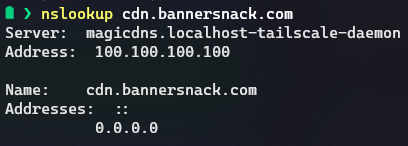
\includegraphics[scale=0.75]{pihole-test.png}
    \caption{Próba znalezienia rekordów dla domeny cdn.bannersnack.com}
    \label{fig:pihole_test}
\end{figure}
\section{Konfiguracja pihole}
Możemy już więc uzyskać dostęp do panelu administracyjnego PiHole przez Tailscale, np. używając stworzonej wewnątrz sieci domeny (u mnie \url{http://pihole.wcyb.wcyb.blizni.uk/}) - powinien nas przywitać ekran logowania (fig. \ref{fig:pihole_login})
\begin{figure}[H]
    \centering
    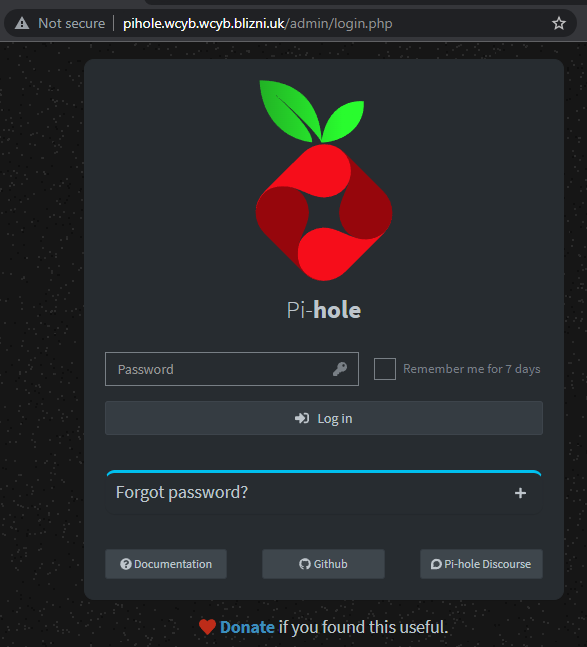
\includegraphics[scale=0.75]{pihole-login.png}
    \caption{Ekran logowania do PiHole}
    \label{fig:pihole_login}
\end{figure}
Po zalogowaniu się stworzonym wcześniej hasłem powinniśmy zobaczyć panel ze statystykami użycia (fig. \ref{fig:pihole_dashboard})
\begin{figure}[H]
    \centering
    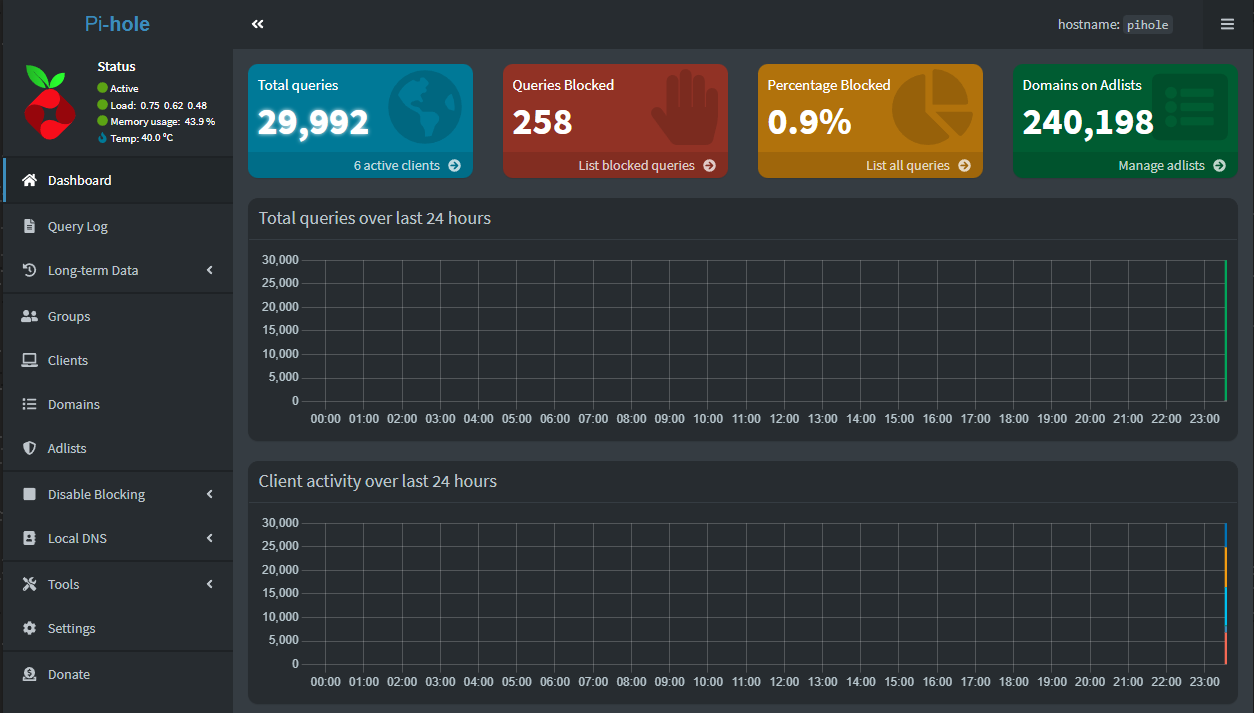
\includegraphics[scale=0.5]{pihole-dashboard.png}
    \caption{Główna strona panelu PiHole}
    \label{fig:pihole_dashboard}
\end{figure}
W panelu jesteśmy w stanie modyfikować część ustawień pihole, manualnie dodawać filtrowane domeny lub wyjątki, dodawać nowe lokalne wpisy DNS, a także aktualizować listy blokowanych domen. Przykładowo dodałem kilka list związanych z bezpieczeństwem (cert.pl, abuse.ch, stopforumspam)
\begin{figure}[H]
    \centering
    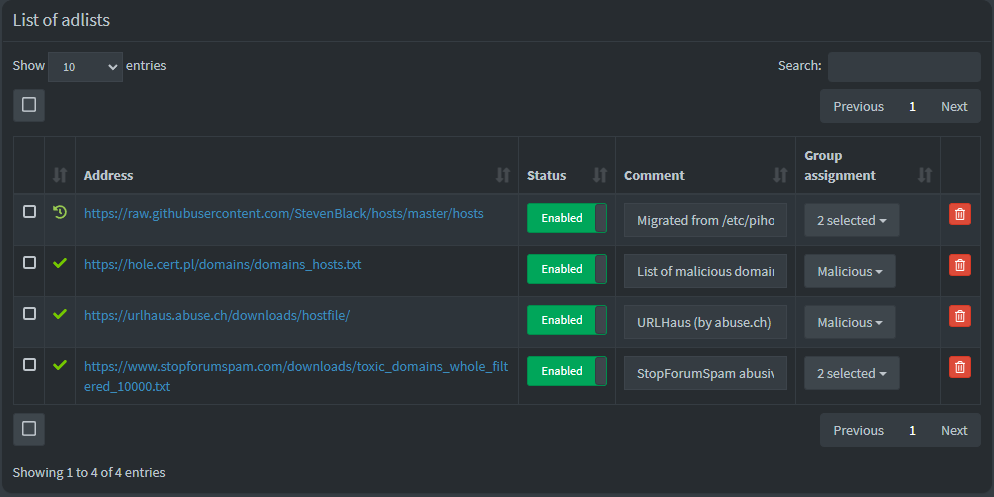
\includegraphics[scale=0.6]{pihole-adlists.png}
    \caption{Listy blokowanych domen w panelu pihole}
    \label{fig:pihole_adlists}
\end{figure}

\section{Podsumowanie}
\subsection{DNS a prywatność}
Operując nawet przez chwilę własny DNS z pełnym logowaniem włączonym nie trudno zauważyć problemu prywatności. Operator jest w stanie prześledzić w zasadzie wszystkie strony do których się łączymy - nawet jeśli nie zna ścieżek na które wchodzimy i nie widzi innych danych żądań, samo to gdzie dany host się łączy stanowi bardzo cenne metadane. A domyślnie wciąż dla większości osób ta masa metadanych trafia do ich operatora internetu, bez żadnego szyfrowania po drodze.

Jednak przez naturę DNS Pi-hole nie do końca rozwiązuje problem jeśli używamy go samemu - kwerendy trafiają do wyższego w hierarchii serwera DNS, nie zmieniając praktycznie nic z ich perspektywy. Dopiero przy większej ilości użytkowników pojawia się zysk w postaci agregacji kwerend (tj. serwer wyżej widzi kwerendy wszystkich jakby pochodziły z jednego urządzenia), ale warto się zastanowić na ile takiej osobie ufamy (chyba, że każdy użytkownik będzie miał dostęp pozwalający sprawdzić, że logowanie domen nie jest włączone w instalacji Pi-hole).

Ale kwerendy DNS nie są jedynym problemem prywatności który Pi-hole potencjalnie adresuje. Drugim, dla większości użytkowników głównym, są reklamy i trackery. Pi-hole wycina je na poziomie DNS, w praktyce po prostu nie pozwalając komputerowi się komunikować ze źródłem reklam i trackerów, tym samym nie dając możliwości nawet ich pobrania. Nie jest to idealne blokowanie - dalej dodatk w przeglądarce może być dobrym pomysłem - ale trudno się kłócić, że jest to poprawa aspektu prywatności w obecnym świecie profilowanych reklam. Jedynym kontrargumentem może być w zasadzie to, że osoby blokujące wszystko też przekazują jakąś informację o sobie (że obchodzi ich prywatność) lub jest to niewystarczające (co niestety można powiedzieć o każdym rozwiązaniu które nie wpływa znacznie negatywnie na doświadczenia korzystania z internetu).

\subsection{DNS a bezpieczeństwo}

Drugą kwestią blisko powiązaną z prywatnością jest bezpieczeństwo. Choć większości osób to nie dotyczy, metadane które wyciekają w naszej historii DNS mogą być jak najbardziej użyteczne dla atakujących z konkretną osobą jako cel. Poznanie np. jakiej poczty email, sieci społecznościowych, usług chmurowych itp. używa pozwala dobrze wycelować choćby atak phishingowy.

Domyślnie większość osób wciąż korzysta z nieszyfrowanych kwerend DNS (choć przeglądarki zaczynają domyślnie włączać DNS over HTTPS), więc nie tylko atak na dostawcę DNS, ale też samo znalezienie się gdzieś w środku trasy wystarczy by poznać o jakie strony dane urządzenie odpytuje.

Konfiguracja Pi-hole, szczególnie w połaczeniu z tailscale, omija to zagrożenie przesyłając cały ruch do Pi-hole przez szyfrowany tunel Wireguard. Bardzo łatwo też ustawić Pi-hole by korzystało z DNS over HTTPS, w praktyce szyfrując cały nasz ruch po drodze.

Dodatkowo samo blokowanie może mieć pozytywny wpływ na bezpieczeństwo - \href{https://cert.pl/posts/2020/03/ostrzezenia_phishing/}{lista ostrzeżeń cert.pl} na przykład zawiera domeny podejrzane o wyłudzanie danych osobowych lub uwierzytelniających, chroniąc przed phishingiem przez po prostu nie pozwolenie się załadować znanym już niebezpiecznym stronom.

\subsection{Alternatywy}
Nie każdy chce jednak hostować własny software. Niestety unikając tego zdajemy się na zaufanie jakiemuś zewnętrznemu dostawy usług. Jeśli jednak to nam pasuje jesteśmy w stanie uzyskać większość zalet Pi-hole korzystając z \href{https://nextdns.io/}{NextDNS}, czyli konfigurowalnego DNSa w formie SaaS.

Jeśli głównie interesuje nas blokowanie reklam to alternatywą (choć nie tylko, bo można korzystać z tego nawet z Pi-hole) jest po prostu adblocker w przeglądarce - np. \href{https://github.com/gorhill/uBlock}{uBlock Origin}.

\end{document}